

\chapter{Missing DATA Mechanism \& LITERATURE SURVEY} \label{chapter1}

\section{Introduction}

Little and Rubin (2002) \cite{Little2002} group different missing data handling strategies into four categories: Procedures Based on Completely Recorded Units, Weighting Procedures, Imputation-Based Procedures, and Model-Based Procedures \cite{Little2002}. Censored data is often replaced with the lowest value in the sample range or the detection limit of the measuring instrument.
Outliers, if detected, can be excluded by truncating or removing from the data set, or winsorizing the data by replacing it with the nearest non-outlying data point \cite{Hastings1947}. Missing data can use different imputation techniques. In the next section we will review some of the most used state of the art methods.


\section{Types of Missing Data :} 

\subsection{Missing completely at random :}

Missing Completely at Random, MCAR,  refers to the non existence of any relationship between the missingness of the data and the rest of data , The statistical advantage of data that are MCAR is that the analysis remains unbiased. Power may be lost in the design, but the estimated parameters are not biased by the absence of the data.
Missing at random : Missing at random (MAR) is a more of what we usually find in real world data,  and it refers to the dependency between the missingness and the observed variables only. And not missing data.
Missing not at random : If the characteristic  of missing data  is neither MCAR nor MAR, then they fall into the category of missing not at random (MNAR). (i.e. the value of the variable that's missing is related to the reason it's missing)

\section{ State of The art :}
In this section we will present the most practical approaches for our problem depending on the nature of data, different solutions for data imputation depending on the kind of problem Time series Analysis, Maximum Likelihood, Multiple Imputation ,Regression etc. and it is difficult to provide a general solution.

\subsection{Classical methods :}

\subsubsection{Listwise or Case Deletion :} A lot of statistical approaches use this techniques by simply omitting those cases with missing data, it has some obvious advantages like it can be applied to any type of statistical analysis. Also, no special computational methods are required, listwise deletion that requires data to be MCAR in order to avoid bias in the results \cite{listwise}.

\subsubsection{Mean - Mode Substitution :}
 As the name suggests we use the mean value of a variable to impute the missing data values, the hypothesis here is the mean substitution is reasonable estimate for a randomly selected observation from a normal distribution, However this method is biased, and leads to an underestimate of the errors\cite{mean}. 

\subsubsection{Interpolation :}
Interpolation is a commonly used method for missing data problems, as it creates new data points within the range of individual observations. The problem of interpolation can be reduced to the approximation of a ”simpler” function by smoothing a given set of observation using linear, polynomial or piece wise spline functions. 


\subsection{Single Imputation Techniques For Univariate Data :}
Usually in the case of Univariate data , means when we have one variable, i.e Time Series  with one variable ( temperature, pressure…),In single imputation analyses, NA values are estimated/replaced one time with one particular data value for the purpose of obtaining more complete samples, at the expense of creating some potential bias in the eventual conclusions or obtaining slightly less accurate estimates than would be available if there were no missing values in the data.

\subsubsection{Auto-regressive Integrated Moving Average (ARIMA)}
it is  important to understand that ARIMA modelling works only with stationary time series data. A stationary Time Series is one whose properties do not depend on the time it is being observed at .
ARIMA (Auto Regressive Integrated Moving Average) is a class of parametric regression models. In this section we will introduce ARIMA and related methods such as moving averages and autoregressive.
For an in depth understanding of these methods, the reader is encouraged to refer to \cite{tong1990non},\cite{brockwell2006introduction} and \cite{box2015time}.
Trends and seasonality affect time series and hence make it non-stationary. Although this seems as a big restriction, in short term traffic prediction, ARIMA models have been very successful. Two basic models constitute ARIMA models - AR (autoregressive) and MA (moving average).
The main idea behind autoregressive models is that past values affect the present value, i.e. $x_{t}$ can be expressed as a function of past p values $ x_{t-1}, x_{t-2},...,x_{t-p} $ , where p is the number of steps into the past. We can express an autoregressive model of order p as below
        \begin{equation} \label{eq:autoregressive}
          x_{t} = \phi_{1}x_{t-1} + \phi_{2}x_{t-2} + ... + \phi_{p}x_{t-p} + w_{t}
        \end{equation}
where $x_{t}$ is stationary and $\phi_{1}, \phi_{2},..., \phi_{p}$ are constant parameters that are to be chosen. We have added the term $w_{t}$ as a Gaussian white noise with zero mean and variance $\sigma^{2}_{w}$.
In the MA model, the current value is dependent on the last q one-step forecast errors $e_{t-1}, e_{t-2},...,e_{t-q}$ and the white noise $w_{t}$. The expression for moving average Is
        \begin{equation} \label{eq:movingaverage}
          x_{t} = -\theta_{1}e_{t-1} - \theta_{2}e_{t-2} - ... - \theta_{q}e_{t-q} + w_{t}
        \end{equation}

$\theta_{1}, \theta_{2},..., \theta_{q}$ are the parameters to be chosen.
Now proceeding to an ARMA (autoregressive moving average) model, we define an ARMA(p,q) model where the present value $x_{t}$ is dependent on p past recent values and q past recent forecast errors and a white noise $w_{t}$.
        \begin{equation} \label{eq:arma}
          x_{t} = \phi_{1}x_{t-1} + \phi_{2}x_{t-2} + ... + \phi_{p}x_{t-p} - \theta_{1}e_{t-1}
          - \theta_{2}e_{t-2} - ... - \theta_{q}e_{t-q} + w_{t}
        \end{equation}
When q is 0, the model becomes an autoregressive model of order p, AR(p) and when p is 0 the model is a moving average of order q, MA(q). We can rewrite \ref{eq:arma} by using the backshift operator $B^{\alpha}$, which is defined as $B^{\alpha}z_{t} = z_{t-\alpha}$,
        \begin{equation} \label{eq:armarewrite}
          \phi(B)x_{t} = \theta(B)e_{t}
        \end{equation}
where
        \begin{equation}
            \phi(z) = 1 - \phi_{1}z - ... - \phi_{p}z^{p}
        \end{equation}
        \begin{equation}
            \theta(z) = 1 - \theta_{1}z - ... - \theta_{q}z^{q}
        \end{equation}

In practice, most time series data are non-stationary and so several approaches, for instance differencing, are used to make it stationary before applying the ARMA(p,q) model. By combining differencing with autoregressive and moving averages, we obtain the ARIMA model which is defined as below

        \begin{equation} \label{eq:arima}
          x'_{t} = \phi_{1}x'_{t-1} + \phi_{2}x'_{t-2} + ... + \phi_{p}x'_{t-p} -
          \theta_{1}e_{t-1} - \theta_{2}e_{t-2} - ... - \theta_{q}e_{t-q} + w_{t}
        \end{equation}

where $x'_{t}$ is the differenced series. Formally the model is denoted as ARIMA(p,d,q) where p is the order of autoregressive part, d is the degree of differencing and q is the order of moving average. This is also known as a non-seasonal ARIMA model.
The common method used to determine the parameters in an ARIMA(p,d,q) model is known as the Box-Jenkins approach (\cite{box2015time}) which is a three stage procedure. The three stages are identification, estimation and diagnostic checking. At the identification stage, the values p, d and q are determined by observing the autocorrelation and partial autocorrelation functions of the time series and its differences. At the estimation stage, the maximum likelihood estimates are determined for each model parameter. Finally in the diagnostics stage, the residuals are analysed and model comparisons are done. If the model fits well then the standardised residuals behave as an i.i.d. with mean zero and variance one.
\subsubsection{Vector Autoregression (VAR) : }
The vector autoregression (VAR) model extends the idea of univariate autoregression to $k$ time series regressions, where the lagged values of all $k$ series appear as regressors. Put differently, in a VAR model we regress a vector of time series variables on lagged vectors of these variables. As for AR($p$) models, the lag order is denoted by $p$ so the VAR($p$) model of two variables $X_{t}$ and $Y_{t}(k=2)$ is given by the equations  
\begin{align*}
  Y_t =& \, \beta_{10} + \beta_{11} Y_{t-1} + \dots + \beta_{1p} Y_{t-p} + \gamma_{11} X_{t-1} + \dots + \gamma_{1p} X_{t-p} + u_{1t}, \\
  X_t =& \, \beta_{20} + \beta_{21} Y_{t-1} + \dots + \beta_{2p} Y_{t-p} + \gamma_{21} X_{t-1} + \dots + \gamma_{2p} X_{t-p} + u_{2t}.
\end{align*}
The $\beta_{s}$ and  $\gamma_{s}$ can be estimated using OLS on each equation.\\Usually this VAR is a good forecasting method for Multivariate Time Series data.

\subsection{Machine learning \& Deep Learning approaches :}


\subsection{Adaboost :}


AdaBoost \cite{adaboost}is an iterative algorithm.
In a given step $m$, we use a weak learner $h(\cdot)$ to estimate a classifier $\hat{h}^{[m]}(\cdot)$, that minimizes the weighted sum of misclassified points.
Based on the misclassification rate a weight $\alpha^{[m]}$ is assigned to the classifier $\hat{h}^{[m]}(\cdot)$.
After a first iteration, the classifier is $F^{[1]}(\cdot)=\hat{\alpha}^{[1]}\hat{h}^{[1]}(\cdot)$.
Using this initial classifier, some points will be correctly classified, and some will be misclassified.
We calculate the errors and change the weights of the misclassified ones, and normalize the weights afterwards, to ensure that the sum of the weights is always the same.
This results in the correctly classified observations having a reduced weight, and with misclassified observations having an increased weight.
In the following iteration, we apply again a weak learner which minimizes the weighted sum of the observations, and we reweight the observations accordingly, in the same manner as before.
Again, calculate a weight to give to this new classifier, and add it to the previous classifier, such that $F^{[2]}(x)=\hat{\alpha}^{[1]}\hat{h}^{[1]}(x)+\alpha^{[2]}h^{[2]}(x)$
Continue iterating in this fashion until an iteration number $\mstop$ is reached.
The resulting AdaBoost classifier $\hat{F}(\cdot)$ becomes
\begin{equation*}
    \hat{F}(x)=F^{[m]}(x)=\sum_{m=1}^{\mstop}\hat{\alpha}^{[m]}\hat{h}^{[m]}(x),
\end{equation*}

i.e. a linear combination of the weak classifiers, or in essence a weighted majority vote of weak learners given the observations.

The AdaBoost algorithm often carries out highly accurate prediction.
In practice, it is often used with stumps, which are decision trees with one split.

in our use case of this approach we will use the regression version.


\subsection{Recurrent Neural Networks :}
Recurrent Neural networks (RNNs) they were based on the work of  David Rumelhart \cite{} (based on wikipedia references) these Neural networks  well suited for sequential  data, They are consider the state of the art now for Natural Language Processing, Especially Machine translation \citet{} and Speech recognition \citet{} with the ability to capture temporal dependencies between variables, a simple Artificial neural network is able to learn linearity and even non linear functions with enough trainign examples, but one thing it can not perform is inculding the time in their learning.  RNNs have been used in many time series applications including126speech recognition (?), electricity forecasting (?)  and weather forecasting.
A recurrent neural network is a feed forward neural network with additional connections between the nodes in each hidden layer called recurrent connections. These recurrent connections, connect the weighted output of each hidden node to another hidden node across a single time step. It is important to note that these recurrent connections do not form cycles within a single time step. The weights carried by these recurrent edges represent state that is remembered from one time step to the next and it is through this state that the recurrent neural network learns to infer context\cite{DBLP:journals/corr/Lipton15}.
Figure \ref{fig:recurrent-neural-network} (a) shows a recurrent neural network with one input unit, one output unit and a hidden layer with two units. It also shows the recurrent connections in the hidden layer. Each node in the hidden layer receives inputs from the data point $x$ and from each hidden unit $h$ in the previous time step. Figure \ref{fig:recurrent-neural-network} (b) show the same recurrent neural network that is unfolded into two time steps. Notice that the recurrent connections are no longer depicted as cyclic connections.

\subsubsection{Recurrent Neural Networks}
\begin{figure}
\centering	
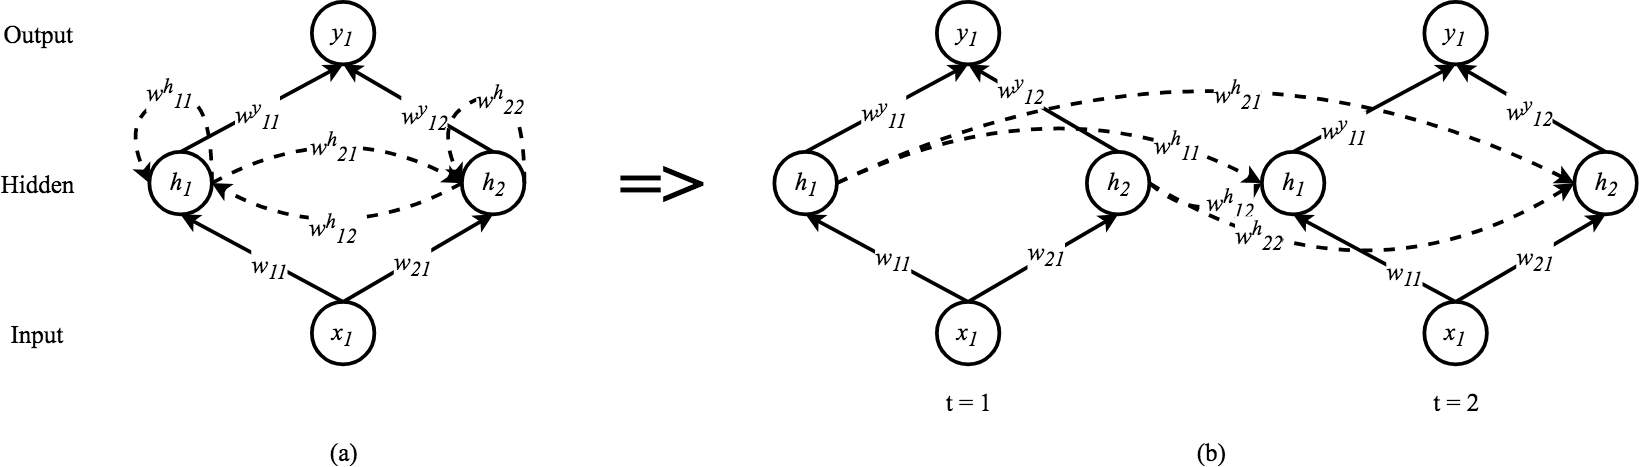
\includegraphics[width=0.8\textwidth]{recurrent-neural-network}
\caption{A recurrent neural network with one hidden layer consisting of two units (a). The same neural network in (a) that is unfolded into two time steps (b).}
\label{fig:recurrent-neural-network}
\end{figure}
%%%%%%%%%%%%%%%%%%%%%%

\subsubsection{Long Short-Term Memory Units}
RNNs encounter difficulties when modeling arbitrary long sequences. When training RNNs on longer sequences the internal weights become too small to be able to capture any context. This is know as the vanishing gradient problem and long short-term memory units (LSTMs) were introduced to overcome this problem\cite{DBLP:journals/corr/Lipton15}. LSTMs employ gating elements that select which parts of the context the unit should "remember" and the parts that it should "forget"\cite{LSTM}.
The use of LSTM in RNN architecture allows long term dependencies in data to be remembered within the model \citep{Graves2013a}, a feature that can be exploited to predict the next value of the sequence. If the predicted value is equal to or within a reasonable range of the observed value, the observed value can be assumed to be valid. The observed value is missing or fails an outlier test, the predicted value replaces the missing value and becomes part of the input to the next sequence test.